\documentclass{article}
\usepackage{tikz}
\usepackage{amsmath}
\usetikzlibrary{patterns}

\begin{document}

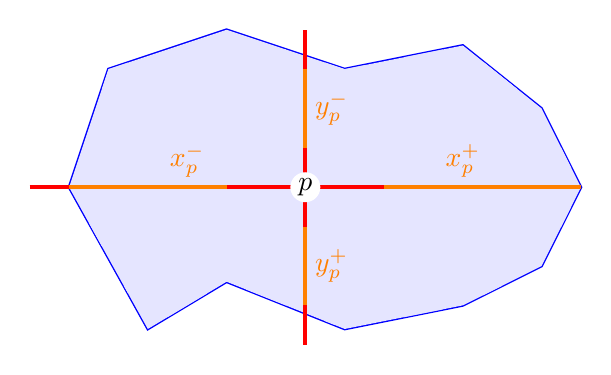
\begin{tikzpicture}
% Define the pattern for poorly textured region
\begin{scope}
    % Create an irregular blue boundary shape
    \draw[blue, line width=1pt] 
        (-3,0) -- (-2.5,1.5) -- (-1,2) -- (0.5,1.5) -- (2,1.8) -- (3,1) -- 
        (3.5,0) -- (3,-1) -- (2,-1.5) -- (0.5,-1.8) -- (-1,-1.2) -- (-2,-1.8) -- (-3,0);
    
    % Fill with checkered pattern
    \clip 
        (-3,0) -- (-2.5,1.5) -- (-1,2) -- (0.5,1.5) -- (2,1.8) -- (3,1) -- 
        (3.5,0) -- (3,-1) -- (2,-1.5) -- (0.5,-1.8) -- (-1,-1.2) -- (-2,-1.8) -- (-3,0);
    
    % Create a light blue checkered pattern
    \foreach \x in {-3,-2.5,...,3.5}
        \foreach \y in {-2,-1.5,...,2}
            \fill[blue!10] (\x,\y) rectangle (\x+0.5,\y+0.5);
    
    \foreach \x in {-2.75,-1.75,...,3.25}
        \foreach \y in {-1.75,-0.75,...,1.75}
            \fill[blue!10] (\x,\y) rectangle (\x+0.5,\y+0.5);
\end{scope}

% Draw the red cross lines
\draw[red, line width=1.5pt] (0,-2) -- (0,2);
\draw[red, line width=1.5pt] (-3.5,0) -- (3.5,0);

% Draw the orange points/lines
\draw[orange, line width=1.5pt] (-3,0) -- (-1,0);
\draw[orange, line width=1.5pt] (1,0) -- (3.5,0);
\draw[orange, line width=1.5pt] (0,-1.5) -- (0,-0.5);
\draw[orange, line width=1.5pt] (0,0.5) -- (0,1.5);

% Add labels
\node at (0,0) [circle, fill=white, inner sep=1pt] {$p$};
\node at (-1.5,0) [above, orange] {$x_p^-$};
\node at (2,0) [above, orange] {$x_p^+$};
\node at (0,1) [right, orange] {$y_p^-$};
\node at (0,-1) [right, orange] {$y_p^+$};

\end{tikzpicture}

\end{document}